%% 
%% Copyright 2007-2020 Elsevier Ltd
%% 
%% This file is part of the 'Elsarticle Bundle'.
%% ---------------------------------------------
%% 
%% It may be distributed under the conditions of the LaTeX Project Public
%% License, either version 1.2 of this license or (at your option) any
%% later version.  The latest version of this license is in
%%    http://www.latex-project.org/lppl.txt
%% and version 1.2 or later is part of all distributions of LaTeX
%% version 1999/12/01 or later.
%% 
%% The list of all files belonging to the 'Elsarticle Bundle' is
%% given in the file `manifest.txt'.
%% 
%% Template article for Elsevier's document class `elsarticle'
%% with harvard style bibliographic references

\documentclass[preprint,12pt,authoryear]{elsarticle}

%% Use the option review to obtain double line spacing
%% \documentclass[authoryear,preprint,review,12pt]{elsarticle}

%% Use the options 1p,twocolumn; 3p; 3p,twocolumn; 5p; or 5p,twocolumn
%% for a journal layout:
%% \documentclass[final,1p,times,authoryear]{elsarticle}
%% \documentclass[final,1p,times,twocolumn,authoryear]{elsarticle}
%% \documentclass[final,3p,times,authoryear]{elsarticle}
%% \documentclass[final,3p,times,twocolumn,authoryear]{elsarticle}
%% \documentclass[final,5p,times,authoryear]{elsarticle}
%% \documentclass[final,5p,times,twocolumn,authoryear]{elsarticle}

%% For including figures, graphicx.sty has been loaded in
%% elsarticle.cls. If you prefer to use the old commands
%% please give \usepackage{epsfig}

%% The amssymb package provides various useful mathematical symbols
\usepackage{amssymb}
%% The amsmath package provides various useful equation environments.
\usepackage{amsmath}
%% The amsthm package provides extended theorem environments
%% \usepackage{amsthm}
\usepackage{hyperref}

%% The lineno packages adds line numbers. Start line numbering with
%% \begin{linenumbers}, end it with \end{linenumbers}. Or switch it on
%% for the whole article with \linenumbers.
%% \usepackage{lineno}

\journal{Astronomy and Computing}

\begin{document}

\begin{frontmatter}

%% Title, authors and addresses

%% use the tnoteref command within \title for footnotes;
%% use the tnotetext command for theassociated footnote;
%% use the fnref command within \author or \affiliation for footnotes;
%% use the fntext command for theassociated footnote;
%% use the corref command within \author for corresponding author footnotes;
%% use the cortext command for theassociated footnote;
%% use the ead command for the email address,
%% and the form \ead[url] for the home page:
%% \title{Title\tnoteref{label1}}
%% \tnotetext[label1]{}
%% \author{Name\corref{cor1}\fnref{label2}}
%% \ead{email address}
%% \ead[url]{home page}
%% \fntext[label2]{}
%% \cortext[cor1]{}
%% \affiliation{organization={},
%%            addressline={}, 
%%            city={},
%%            postcode={}, 
%%            state={},
%%            country={}}
%% \fntext[label3]{}

\title{Optimizing Effective Temperature Estimation for Eclipsing Binaries using Gaia DR3 Photometry and Ensemble Machine Learning}

%% use optional labels to link authors explicitly to addresses:
%% \author[label1,label2]{}
%% \affiliation[label1]{organization={},
%%             addressline={},
%%             city={},
%%             postcode={},
%%             state={},
%%             country={}}
%%
%% \affiliation[label2]{organization={},
%%             addressline={},
%%             city={},
%%             postcode={},
%%             state={},
%%             country={}}

\author[1]{Author Name\corref{cor1}}
\ead{author@email.com}
\cortext[cor1]{Corresponding author}

\affiliation[1]{organization={Department of Astronomy},%Department and Organization
            addressline={Address}, 
            city={City},
            postcode={Zip}, 
            state={State},
            country={Country}}

\begin{abstract}
Eclipsing binaries (EBs) are fundamental benchmarks for stellar physics, yet a significant fraction of the ~2.5 million EBs in Gaia DR3 lack effective temperature ($T_{\rm eff}$) estimates or possess low-confidence parameters. 
This work presents a comprehensive machine learning framework to predict $T_{\rm eff}$ for approximately 800000 EBs using exclusively Gaia DR3 photometry ($G, BP, RP$). 
We initially explore multi-survey enrichment (SDSS, 2MASS) but prioritise a Gaia-only approach to maximise catalog coverage.
We implement and compare four distinct modeling strategies: 
(1) a Random Forest (RF) regressor trained on high quality GSP-Phot temperatures, 
(2) a RF regressor trained on log-transformed temperatures, 
(3) a model incorporating predicted surface gravity ($\log g$), 
and (4) a structure-augmented model leveraging unsupervised clustering of the colour space. 
We introduce a "Best-of-Four" ensemble method that dynamically selects the prediction with the lowest internal model uncertainty for each source. 
Our final catalog achieves a mean uncertainty of 203 K, significantly improving coverage and reliability for eclipsing binary research.
\end{abstract}

%%Graphical abstract
%\begin{graphicalabstract}
%\includegraphics{grabs}
%\end{graphicalabstract}

%%Research highlights
%\begin{highlights}
%\item Research highlight 1
%\item Research highlight 2
%\end{highlights}

\begin{keyword}
Eclipsing Binaries \sep Gaia \sep Machine Learning \sep Effective Temperature \sep Ensemble Methods
%% keywords here, in the form: keyword \sep keyword
%% PACS codes here, in the form: \PACS code \sep code
%% MSC codes here, in the form: \MSC code \sep code
%% or \MSC[2008] code \sep code (2000 is the default)
\end{keyword}

\end{frontmatter}

%% \linenumbers

%% main text

\section{Introduction}
\label{sec:intro}

Eclipsing binaries (EBs) serve as fundamental pillars of modern astrophysics, offering one of the few direct methods to measure stellar masses and radii with high precision \citep{Andersen1991, Torres2010}. 
As geometric distance indicators and stringent tests for stellar evolution models, their accurate characterisation is essential for calibrating the cosmic distance scale and understanding stellar structure. 
With the eclipsing binaries catalog release of Gaia Data Release 3 (DR3) \citep{GaiaDR3_EB}, the astronomical community has gained access to a catalog of over 2 million identified eclipsing binaries, representing an order-of-magnitude increase over previous compilations.

Traditionally, the precise determination of stellar parameters for eclipsing binaries requires a combination of multi-band photometric light curves and radial velocity measurements from spectroscopy. 
Modeling the light curves yields geometric parameters (relative radii, inclination) and radiative properties (temperature ratios), while radial velocities constrain the absolute scale (masses, semi-major axis). 
The effective temperatures of the individual components are typically anchored by spectroscopic analysis of the composite spectrum or by colour indices calibrated against standard stars. 
Several sophisticated codes have been developed to facilitate this modeling process, such as Wilson-Devinney (WD) code \citep{Wilson1971}, JKTEBOP \citep{Southworth2008}, PHOEBE (Physics Of Eclipsing Binaries) \citep{Prsa2005, Prsa2016}, ELISa \citep{Cokina2021}, and TEB (Temperatures for EB) \citep{Miller2020}. 
However, this comprehensive approach is resource-intensive and limited to relatively bright systems with extensive observational follow-up. 
For large-scale surveys like Gaia, where only limited photometric epochs or low-resolution spectra may be available for millions of targets, these rigorous methods are computationally prohibitive or data-limited.
Nethertheless, the General Stellar Parameteriser from Photometry (GSP-Phot) \citep{GSPphot} provides parameters for approximately 1.2 million sources from Gaia EB catalog: $T_{\rm eff}$, $logg$, and $Fe/H$ values.
Nearly half of the catalog ($\sim$800,000 objects) lacks any estimates. 

To bridge this gap, we turn to machine learning (ML) solutions, which are well-suited to model high-dimensional, non-linear relationships in large datasets. 
This work addresses the limitation by developing a homogeneous, high-coverage $T_{\rm eff}$ catalog for eclipsing binaries using ML techniques applied to Gaia DR3 photometry. 
Our primary objective is to maximise the utility of the existing photometric data ($G, BP, RP$) to predict temperatures for the $\sim$800,000 sources where GSP-Phot data is unavailable.
We tested different approaches to estimate effective temperatures. 
By leveraging a ``Best-of-Four'' ensemble strategy we significantly extend the available sapmle for EB research.

This work is a part of the project to develop a robust automated pipeline for estimating stellar parameters for EBs using photometry. 
We created a synthetic dataset using ELISa to train models and try to solve the problem. 
We already published the results of classification of EBs using computer vision techniques \citep{Parimucha2025}.
One can find the details about the syntheticdataset there. 
We trained models to predict EB system parameters including $T1_{\rm_eff}/T2_{\rm_eff}$. 
Thus we need to estimate $T_{\rm_eff}$ for one of the components to calculate absolute values for other parameters.

The paper is organized as follows: in Section \ref{sec:data} we describe the data we used to train and test the models.
In Section \ref{sec:methods} we describe the methodology we used to train the models.
In Section \ref{sec:results} we present the results of the models.
In Section \ref{sec:conclusion} we discuss the results and the future work.

\section{Data Selection and Enrichment}
\label{sec:data}

The following section outlines the comprehensive series of experiments on input datasets conducted to optimise the temperature estimation pipeline. 
We evaluated a wide range of data enrichment strategies---including multi-survey cross-matching and extensive feature engineering---to assess their impact on prediction accuracy and catalog completeness. 
The associated GitHub repository documents the full spectrum of these investigations, while this paper focuses on the successful strategies that constitute our final "Best-of-Four" ensemble. 
The complete end-to-end pipeline, capable of reproducing all training, validation, and prediction steps, is made available in a dedicated branch of the repository, ensuring transparency and reproducibility of our results.

\subsection{Cross-matching with other surveys}
The primary dataset for this study is derived from the Gaia Data Release 3 (DR3) Eclipsing Binary catalog \citep{GaiaDR3_EB}, which contains approximately 2.1 million identified eclipsing systems. 
This represents the largest homogeneous catalog of EBs to date, offering all-sky coverage and precise photometry in the Gaia $G$ (330--1050 nm), ${BP}$ (330--680 nm), and ${RP}$ (630--1050 nm) passbands \citep{GaiaDR3_main}.

To enhance the feature space for temperature prediction, we initially explored enriching the Gaia catalog with multi-wavelength photometry from other large-scale surveys. 
Specifically, we cross-matched the Gaia EB sources with the Pan-STARRS1 (PS1) DR2 catalog \citep{Chambers2017,Magnier2025}. 
It provides $g, r, i, z, y$ photometry. And the Two Micron All Sky Survey (2MASS) \citep{Skrutskie2006}, which offers near-infrared $J, H, K_s$ magnitudes. 
Our hypothesis was that additional passbands will provide valuable leverage for disentangling temperature and extinction, particularly in the near-infrared where the effects of dust are minimized. 
The cross-matching process significantly reduced the sample size (Table \ref{tab:coverage}). 

\begin{table}[htbp]
\centering
\caption{Photometry Coverage and Temperature Availability}
\label{tab:coverage}
\begin{tabular}{l c c c}
\hline
\textbf{Dataset} & \textbf{Total Objects} & \textbf{With GSP-Phot Teff} & \textbf{Can be Predicted} \\
\hline
Gaia DR3 EB Catalog & 2,184,477 & 1,276,166 (58.4\%) & - \\
Gaia ($G, BP, RP$) & 2,123,652 (97.2\%) & 1,276,166 & 847,486 \\
Gaia + Pan-STARRS & 1,130,862 (51.8\%) & 707,821 & 423,041 \\
Gaia + 2MASS & 1,123,471 (51.4\%) & 926,692 & 196,779 \\
Gaia + PS + 2MASS & 647,260 (29.6\%) & 541,925 & 105,335 \\
\hline
\end{tabular}
\end{table}

Requiring detections in all surveys restricted the dataset to a fraction of the original catalog, limiting the generalisability of the final model to the full objects sample. 
To maximise coverage and ensure our predictions are available for the vast majority of Gaia EBs, we prioritized a Gaia-only photometric approach, relying on the $G, BP, RP$ bands and their derived colors.
Neththeless, we trained and validate the models using different combinations of features to find the best performing model.

\subsection{Validation and Correction of Training Labels}
For training our machine learning models, we utilised the effective temperature ($T_{\rm eff}$) estimates provided by the Gaia GSP-Phot pipeline \citep{GSPphot}. 
To assess the reliability of these labels, we compared the GSP-Phot temperatures against high-quality literature catalogs of detached eclipsing binaries (DEBCat) \citep{DEBCat} and overcontact binaries (WUMaCat) \citep{WUMaCat}. 
This comparison revealed a strong overall correlation, validating the use of GSP-Phot values as a training baseline for the bulk of the population. 
However, we identified a systematic bias in the high-temperature regime: for stars with $T_{\rm eff} \gtrsim 10,000$ K, GSP-Phot tends to underestimate the true effective temperature \ref(teff_comparison). 
To mitigate this, we fitted a second-degree polynomial correction to the residuals between the GSP-Phot values and the values from the catalogues \ref{fig:teff_comparison}. 
This correction function was then applied to the training labels and incorporated into our final prediction pipeline to ensure accurate estimates for hotter systems.

\begin{figure}[htbp]
    \centering
    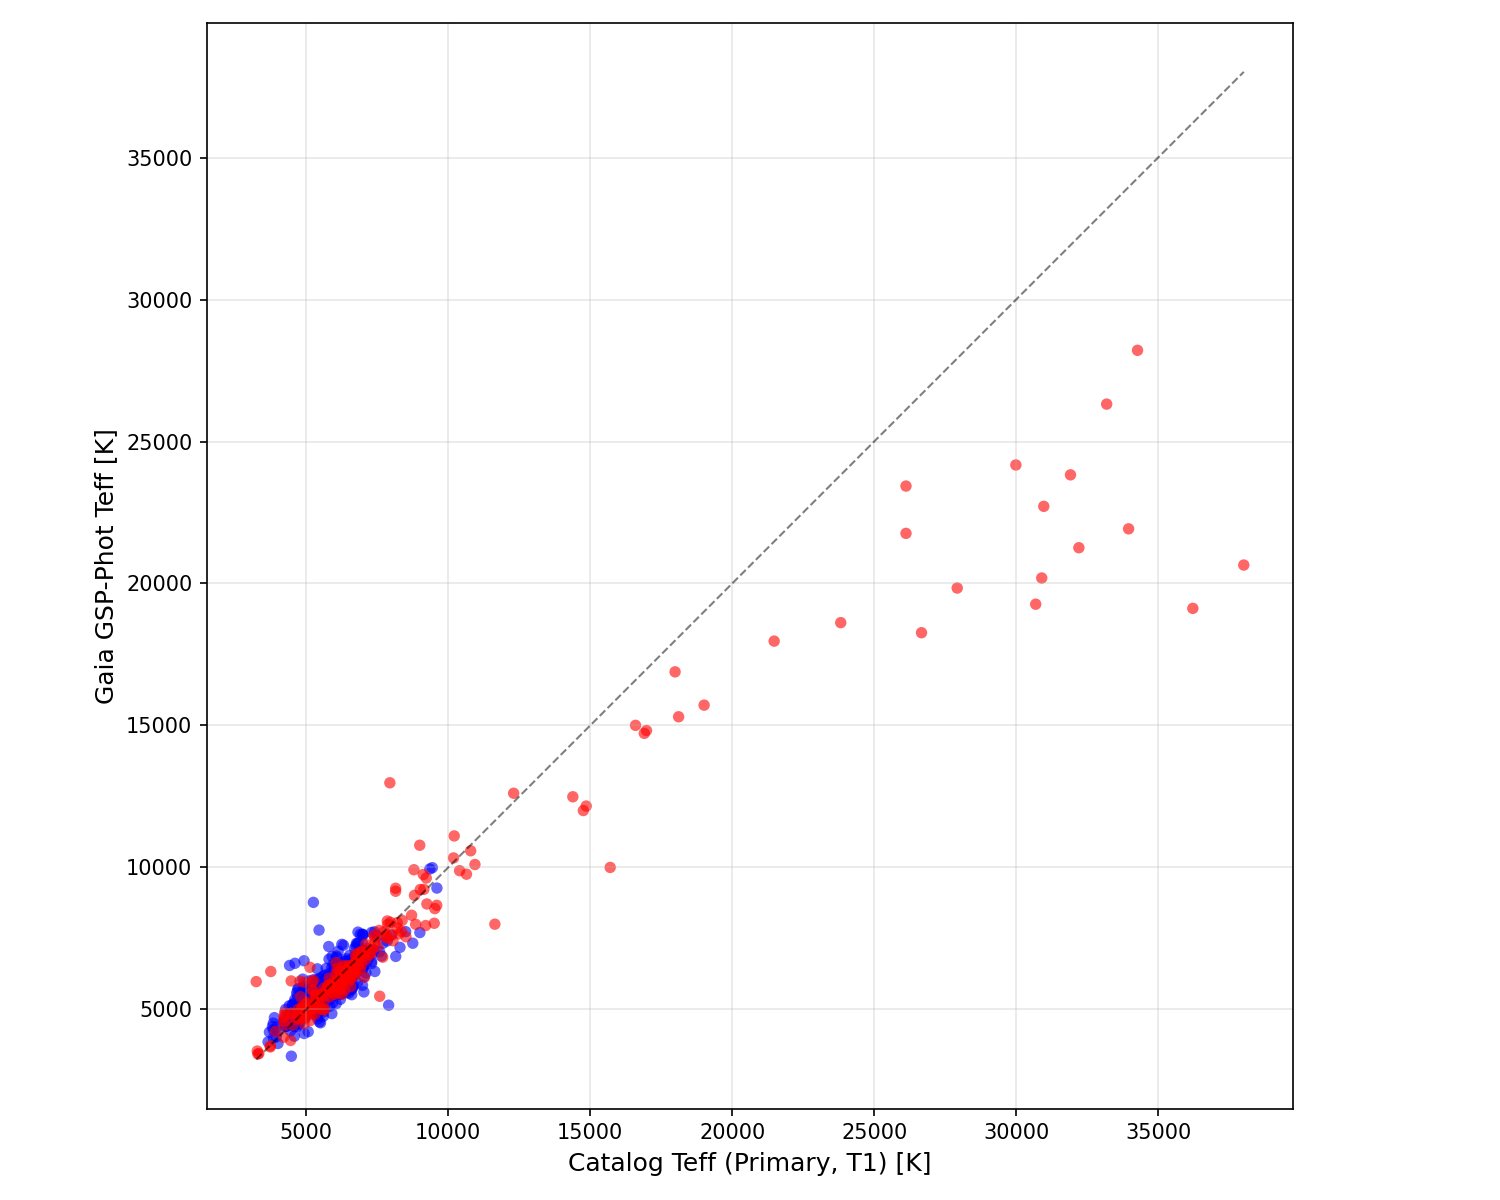
\includegraphics[width=0.48\textwidth]{teff_comparison_T1.png}
    \hfill
    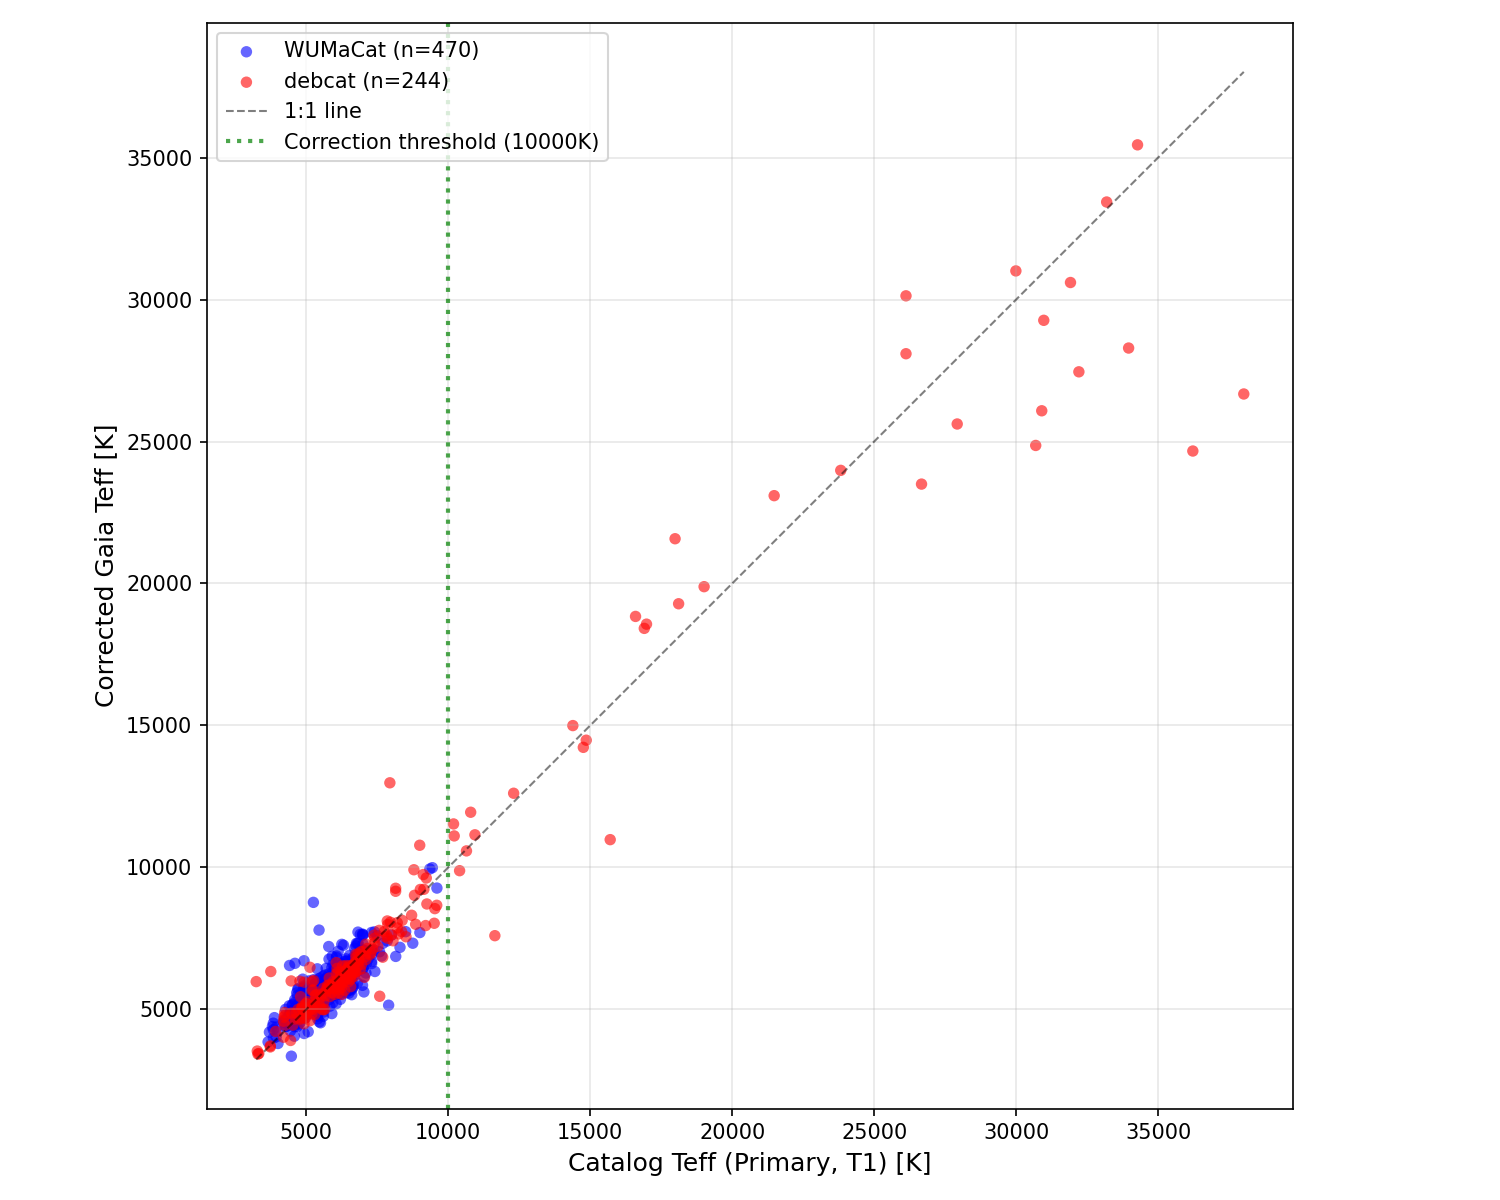
\includegraphics[width=0.48\textwidth]{teff_comparison_t1_corrected_deg2_T1.png}
    \caption{Comparison of effective temperatures. 
    Left: Gaia GSP-Phot temperatures vs. literature values (WUMaCat and DEBCat), showing the deviation for $T_{\rm eff} > 10,000$ K. 
    Right: Corrected Gaia temperatures after polynomial adjustment.}
    \label{fig:teff_comparison}
\end{figure}

It should be mentioned that The distribution of temperatures is highly skewed. 
The number of objects with $T_{\rm eff} > 10,000$ K is relatively small (less than 1\% of the total sample).
Thus we expected that the models will have problems with predicting temperatures for hot stars.
We additionally applied a log-transformation to the temperatures to test how the models will react to a different distribution.

\subsection{Quality Flags}
We utilized the quality flags defined by \cite{Avdeeva2024} for the Gaia DR3 GSP-Phot parameters. 
Their work employs machine learning methods (XGBoost, CatBoost, LightGBM) to classify the reliability of GSP-Phot effective temperatures by comparing them against high-resolution spectroscopic catalogs (APOGEE DR17, GALAH DR3). 
They provide binary quality flags (1 for reliable, 0 for unreliable) that effectively filter out discrepant temperatures, achieving a precision of $\sim$90\% for temperatures accurate to within 250 K. 
We specifically selected objects flagged as ``good'' by their ensemble model to construct a training set free from significant systematic errors and model-dependent artifacts present in the raw GSP-Phot catalog.

\subsection{Feature Engineering}
We expanded our feature space beyond the basic magnitudes and colours. 
We generated polynomial features up to degree 3, interaction terms between all colour pairs, and logarithmic transformations. 
Additionally, we incorporated predictions of surface gravity ($\log g$) from an auxiliary Random Forest model as a physics-informed feature, propagating its prediction uncertainty into the final temperature model.

Furthermore, we introduced unsupervised clustering coefficients as novel features to capture local substructures in the colour space. 
We applied a Gaussian Mixture Model (GMM) \citep{GMM} to the standardised Gaia photometry, clustering the data into 5 distinct components. 
For each object, we calculated the soft membership probabilities for each cluster. 
These probabilities were then included as additional input features for the regression model. 
Our hypothesis was that this approach will allow the Random Forest to learn cluster-specific corrections. 
The temperature prediction on the object's likely evolutionary state or population membership without requiring explicit labels for those states.

\section{Methodology}
\label{sec:methods}

To ensure consistent model performance and manage computational resources effectively, we adopted a two-stage approach to model optimisation. 
Initial experiments to perform a comprehensive grid search for hyperparameter tuning on the full dataset proved computationally prohibitive given the available hardware (2.3 GHz 8-Core Intel Core i9, CPU only). 
Therefore, we determined the optimal hyperparameters (number of trees, maximum depth, minimum samples split/leaf) using a representative subset of the data and varying input feature sets. 
Once established, these hyperparameters ($n_{estimators}=300$, $max_{depth}=20$, $min_{samples\_leaf}=4$) were fixed and applied consistently across all subsequent models to ensure fair comparison of feature engineering strategies.

Additional photometry from different surveys respectively reduced the number of objects in the training set (see Table \ref{tab:coverage}).
Nethertheless the obtained dataset was split into training (80\%) and testing (20\%) subsets using a stratified split to preserve the distribution of the target variable $T_{\rm eff}$. 
For model training, we utilised the Random Forest regressor \citep{RF} from the \texttt{scikit-learn} library. 

Validation of the models was performed using a suite of metrics including Mean Absolute Error (MAE), Root Mean Square Error (RMSE), and the coefficient of determination ($R^2$). 
Additionally, we visually inspected diagnostic plots such as predicted vs. true temperature plots, residual distributions, feature importance rankings to assess model behavior and identify potential biases across different temperature regimes (Figure \ref{fig:four_panel_comparison}).

To have a possibility to compare the confidence of different models on unlabeled data, we leveraged the ensemble nature of Random Forests to estimate prediction uncertainties. 
For every object in the prediction set, we calculated the standard deviation of the predictions from all individual trees in the forest. 
We used those standard deviations as the final uncertainty estimate for the prediction.

\begin{figure}[htbp]
    \centering
    \begin{minipage}{0.48\textwidth}
        \centering
        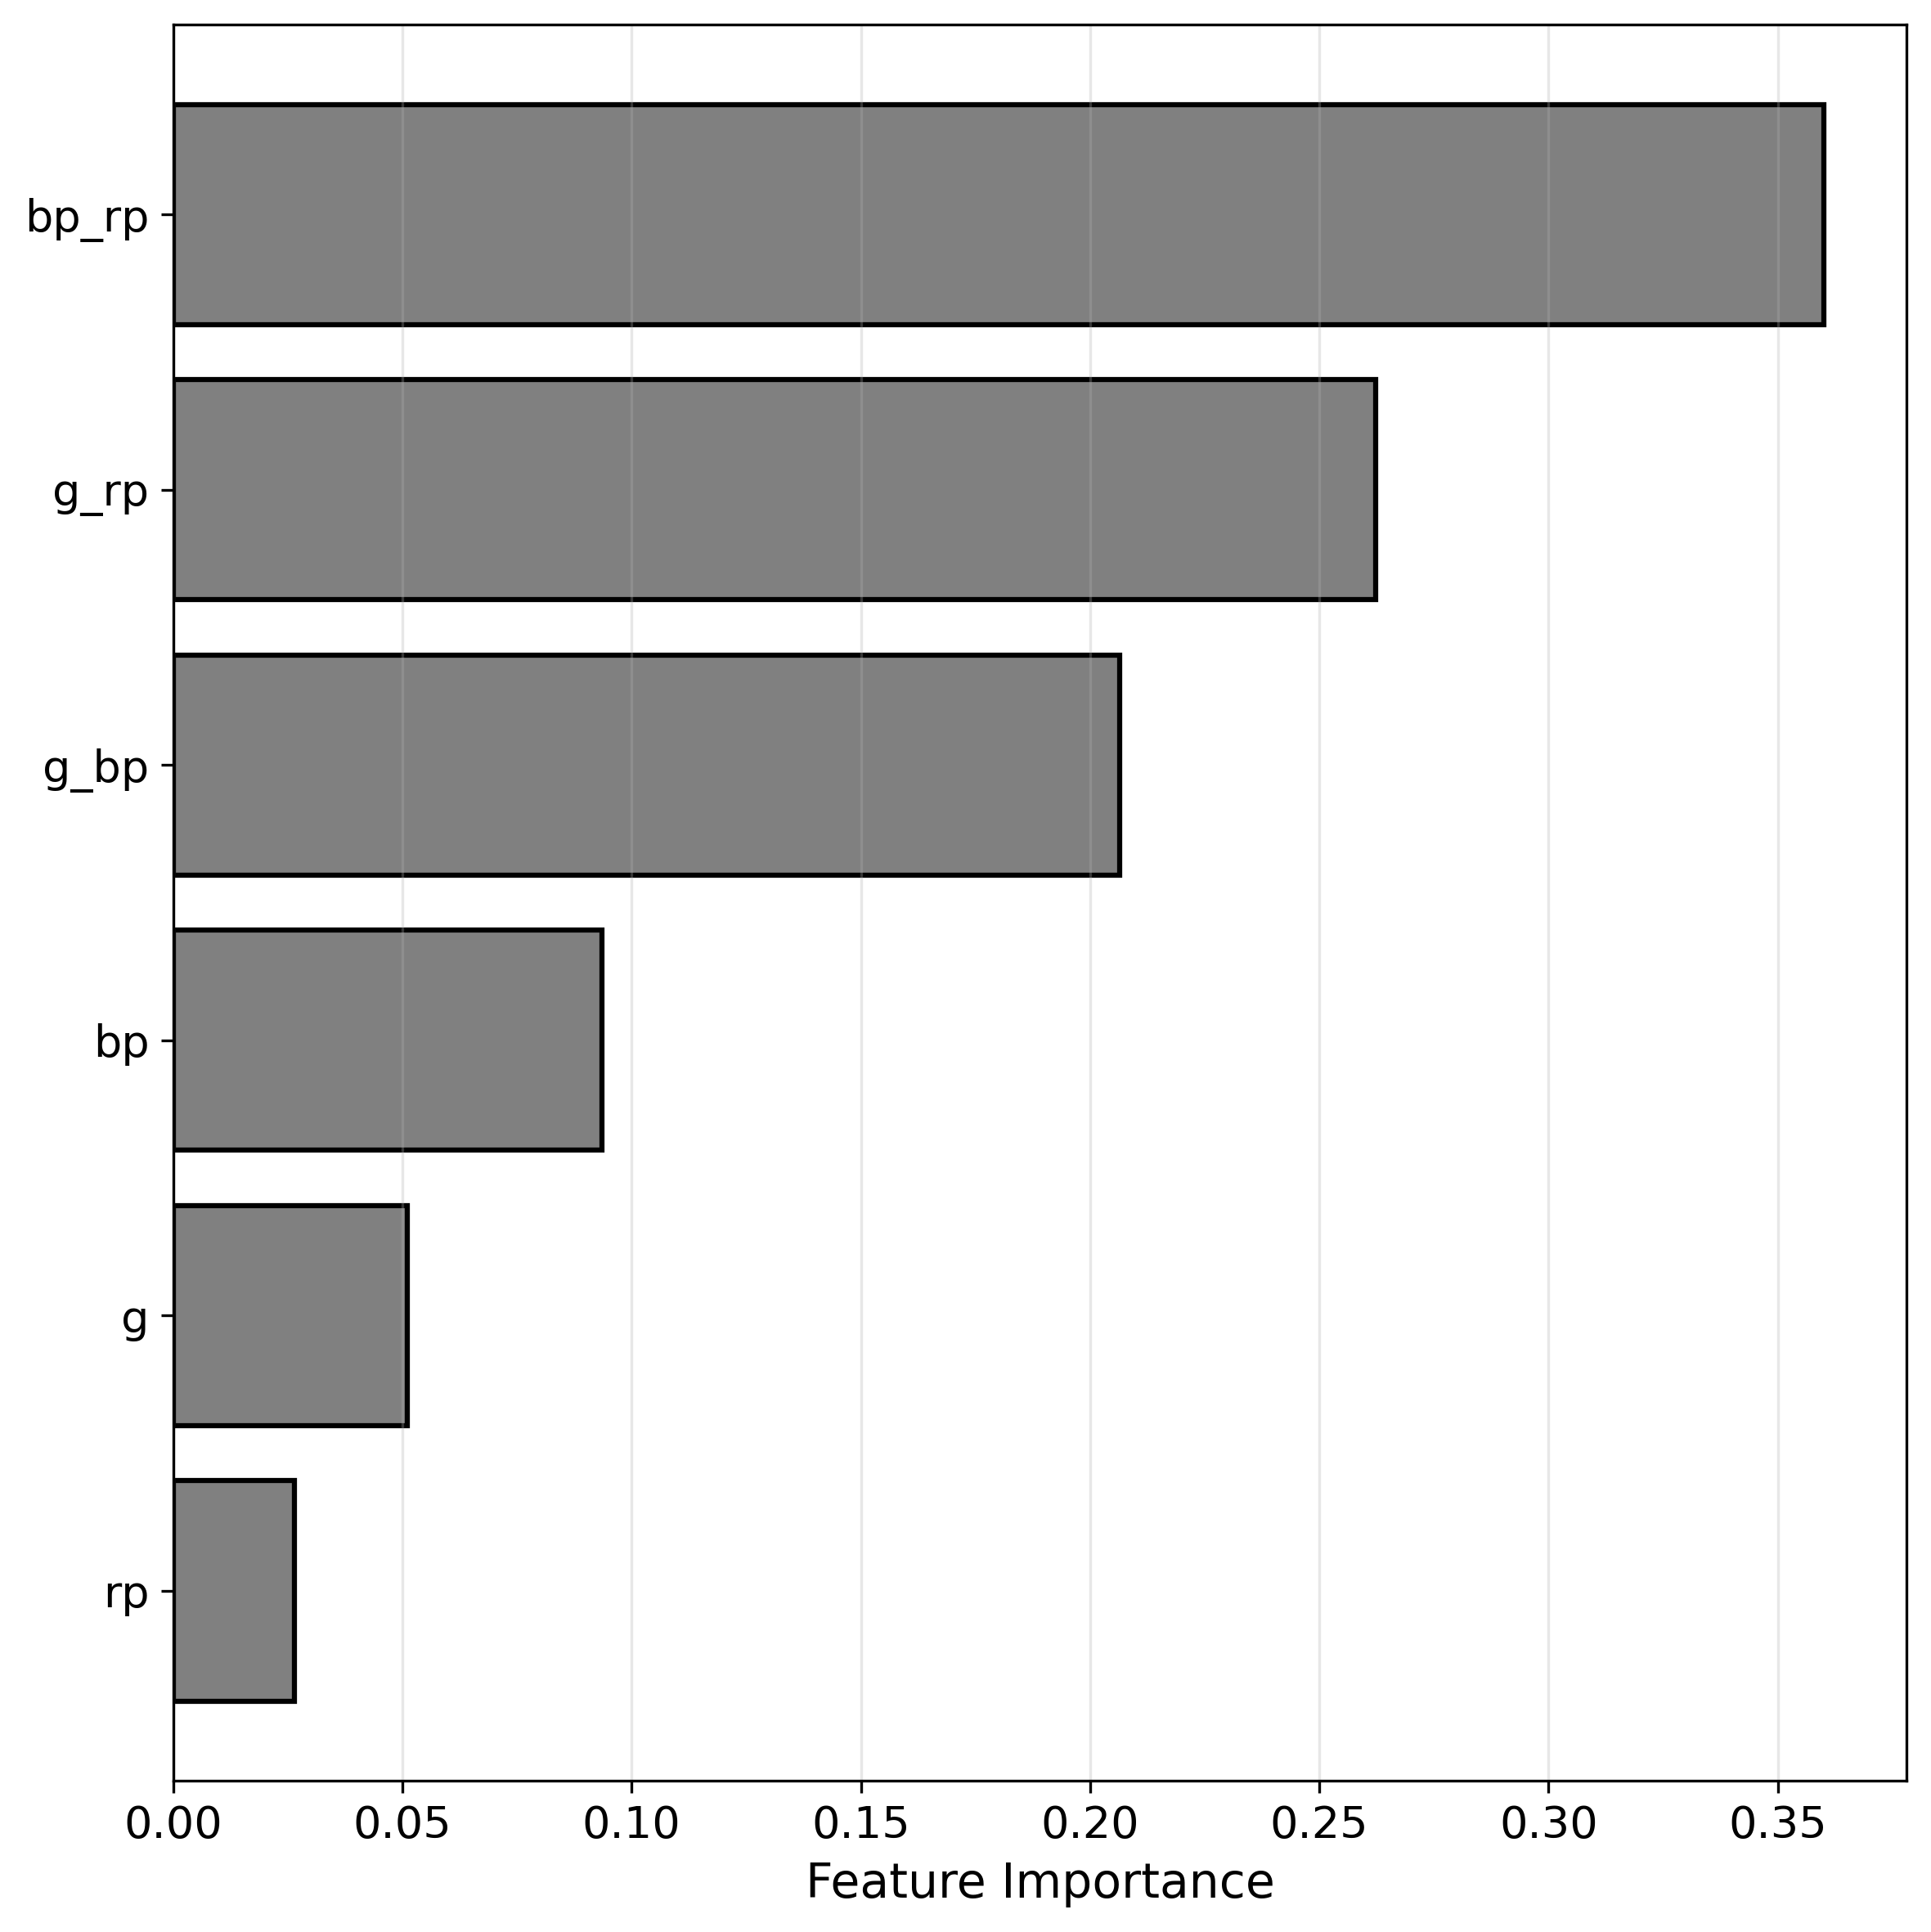
\includegraphics[width=\linewidth]{feature_importance.png} % Replace with first plot
        \label{fig:plot1}
    \end{minipage}\hfill
    \begin{minipage}{0.48\textwidth}
        \centering
        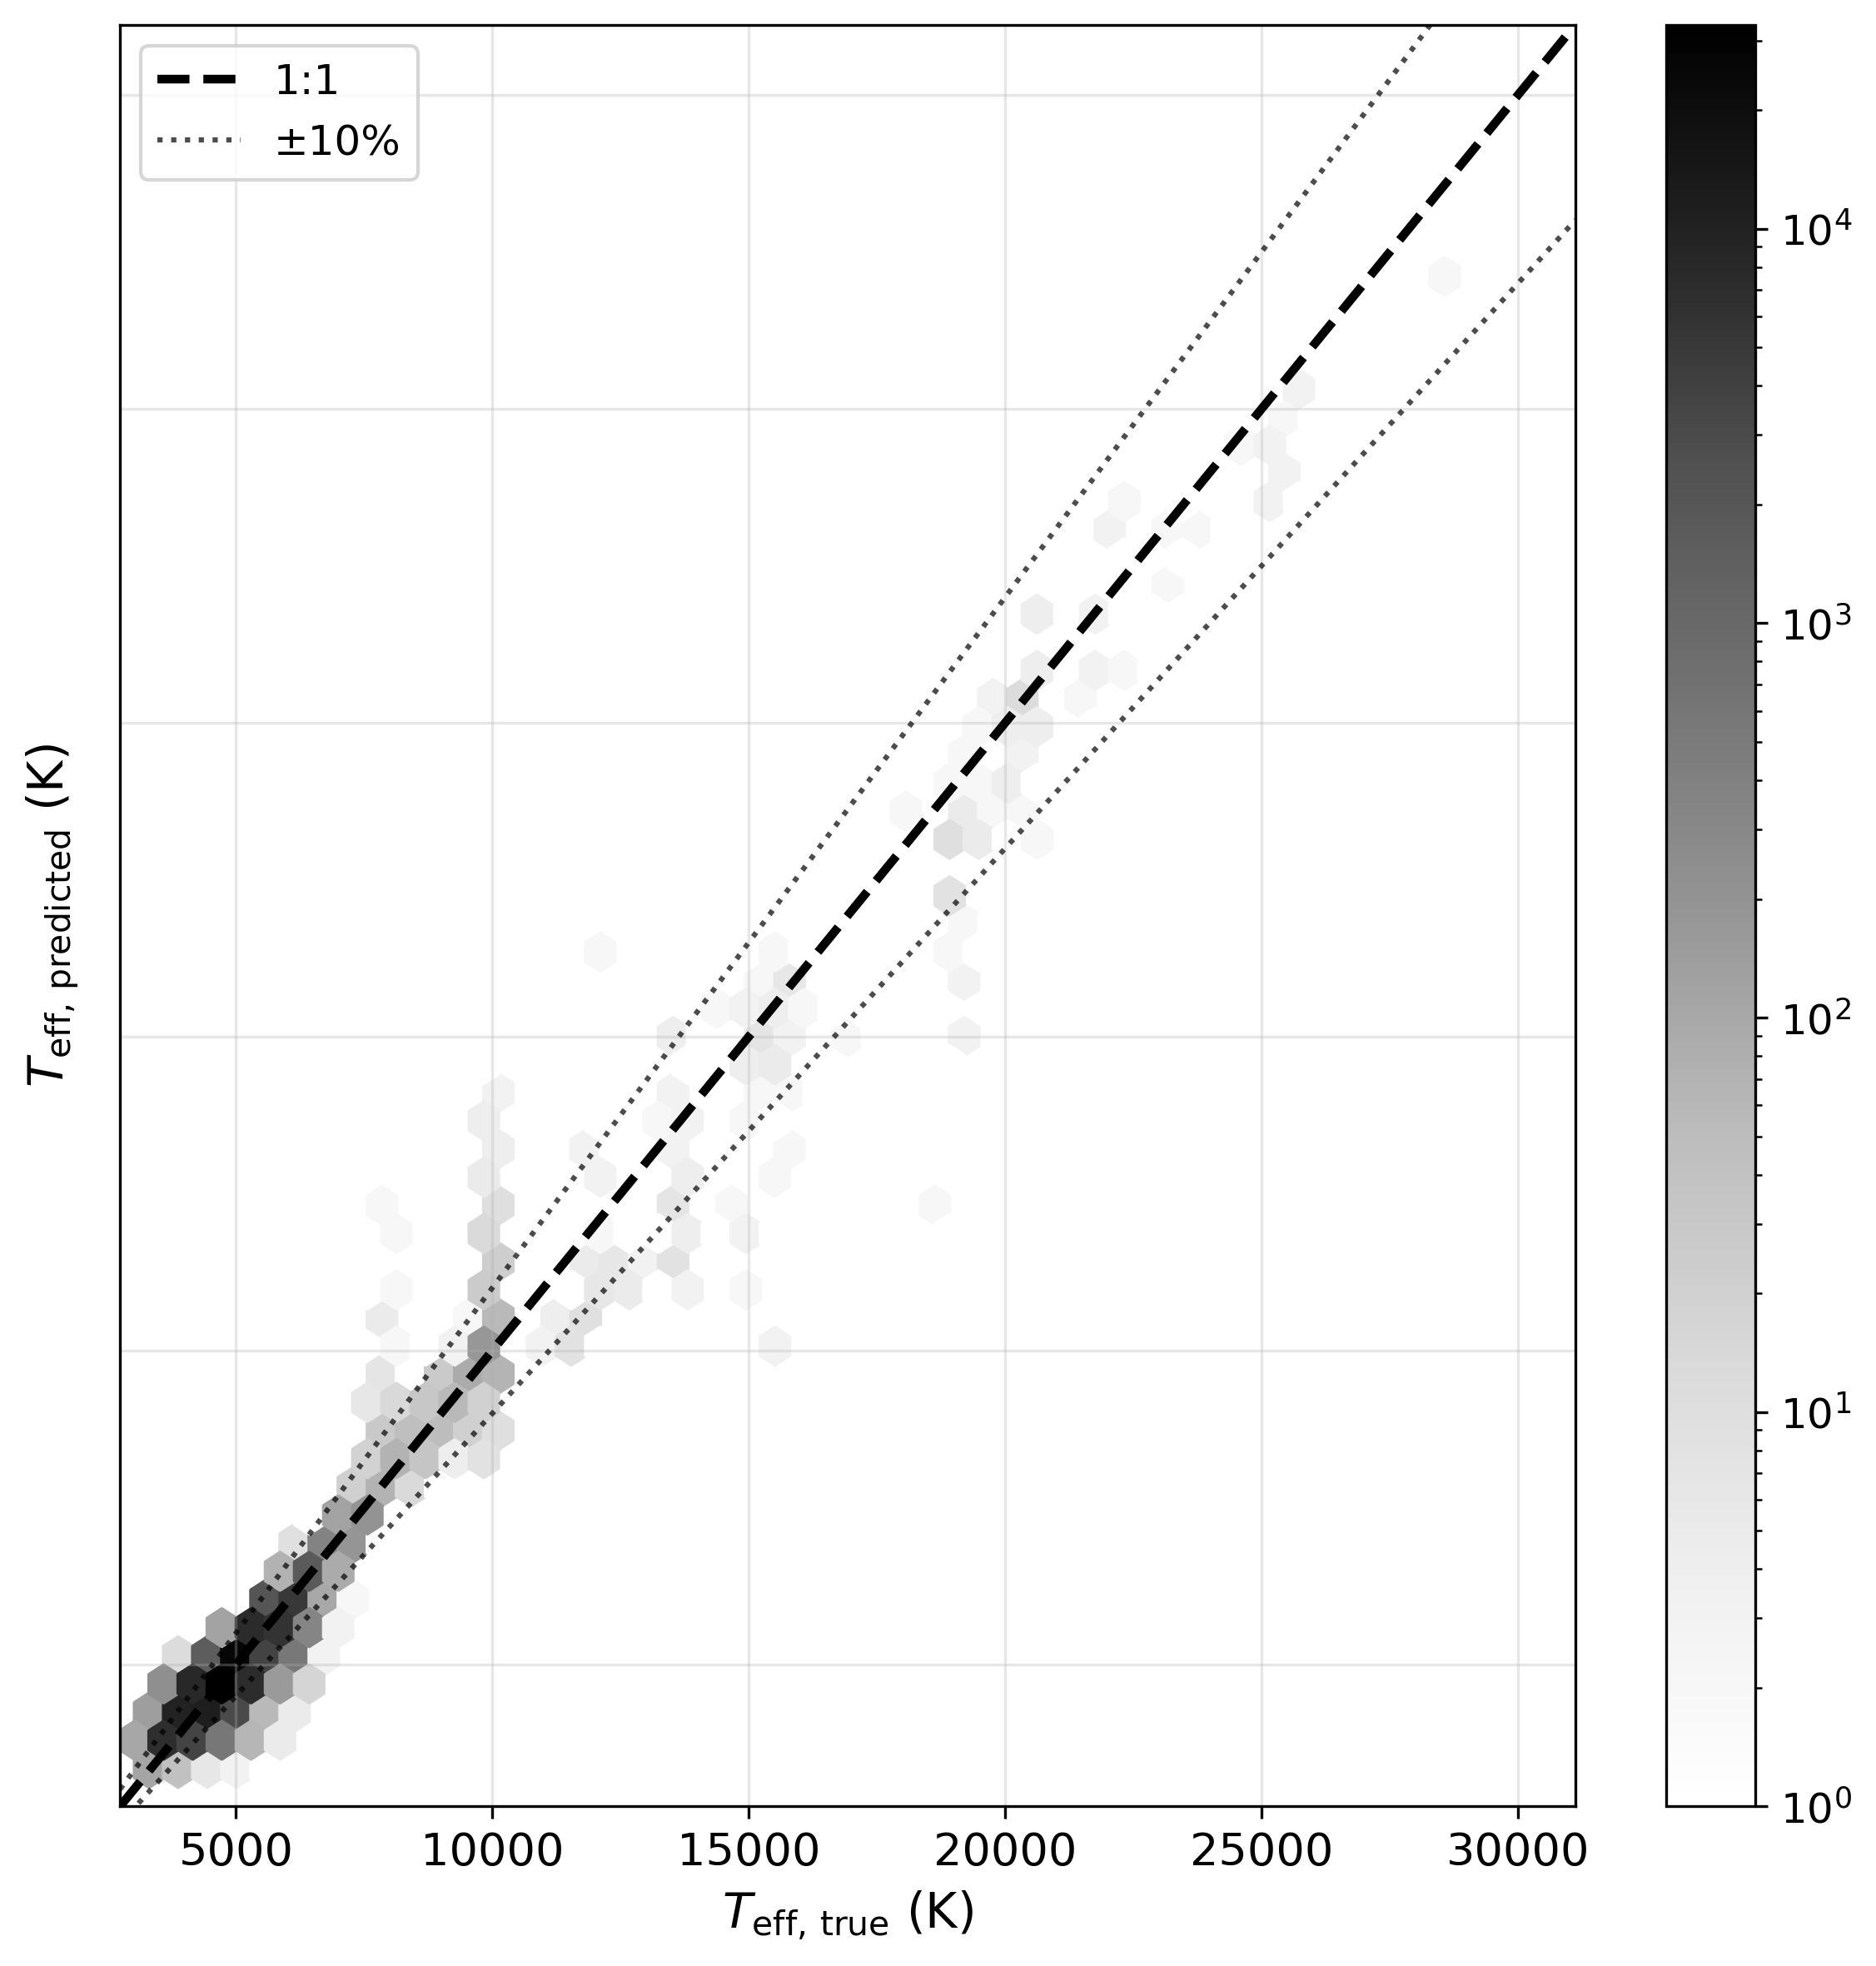
\includegraphics[width=\linewidth]{true_vs_predicted.png} % Replace with second plot
        \label{fig:plot2}
    \end{minipage}
    
    \vspace{0.5cm}
    
    \begin{minipage}{0.48\textwidth}
        \centering
        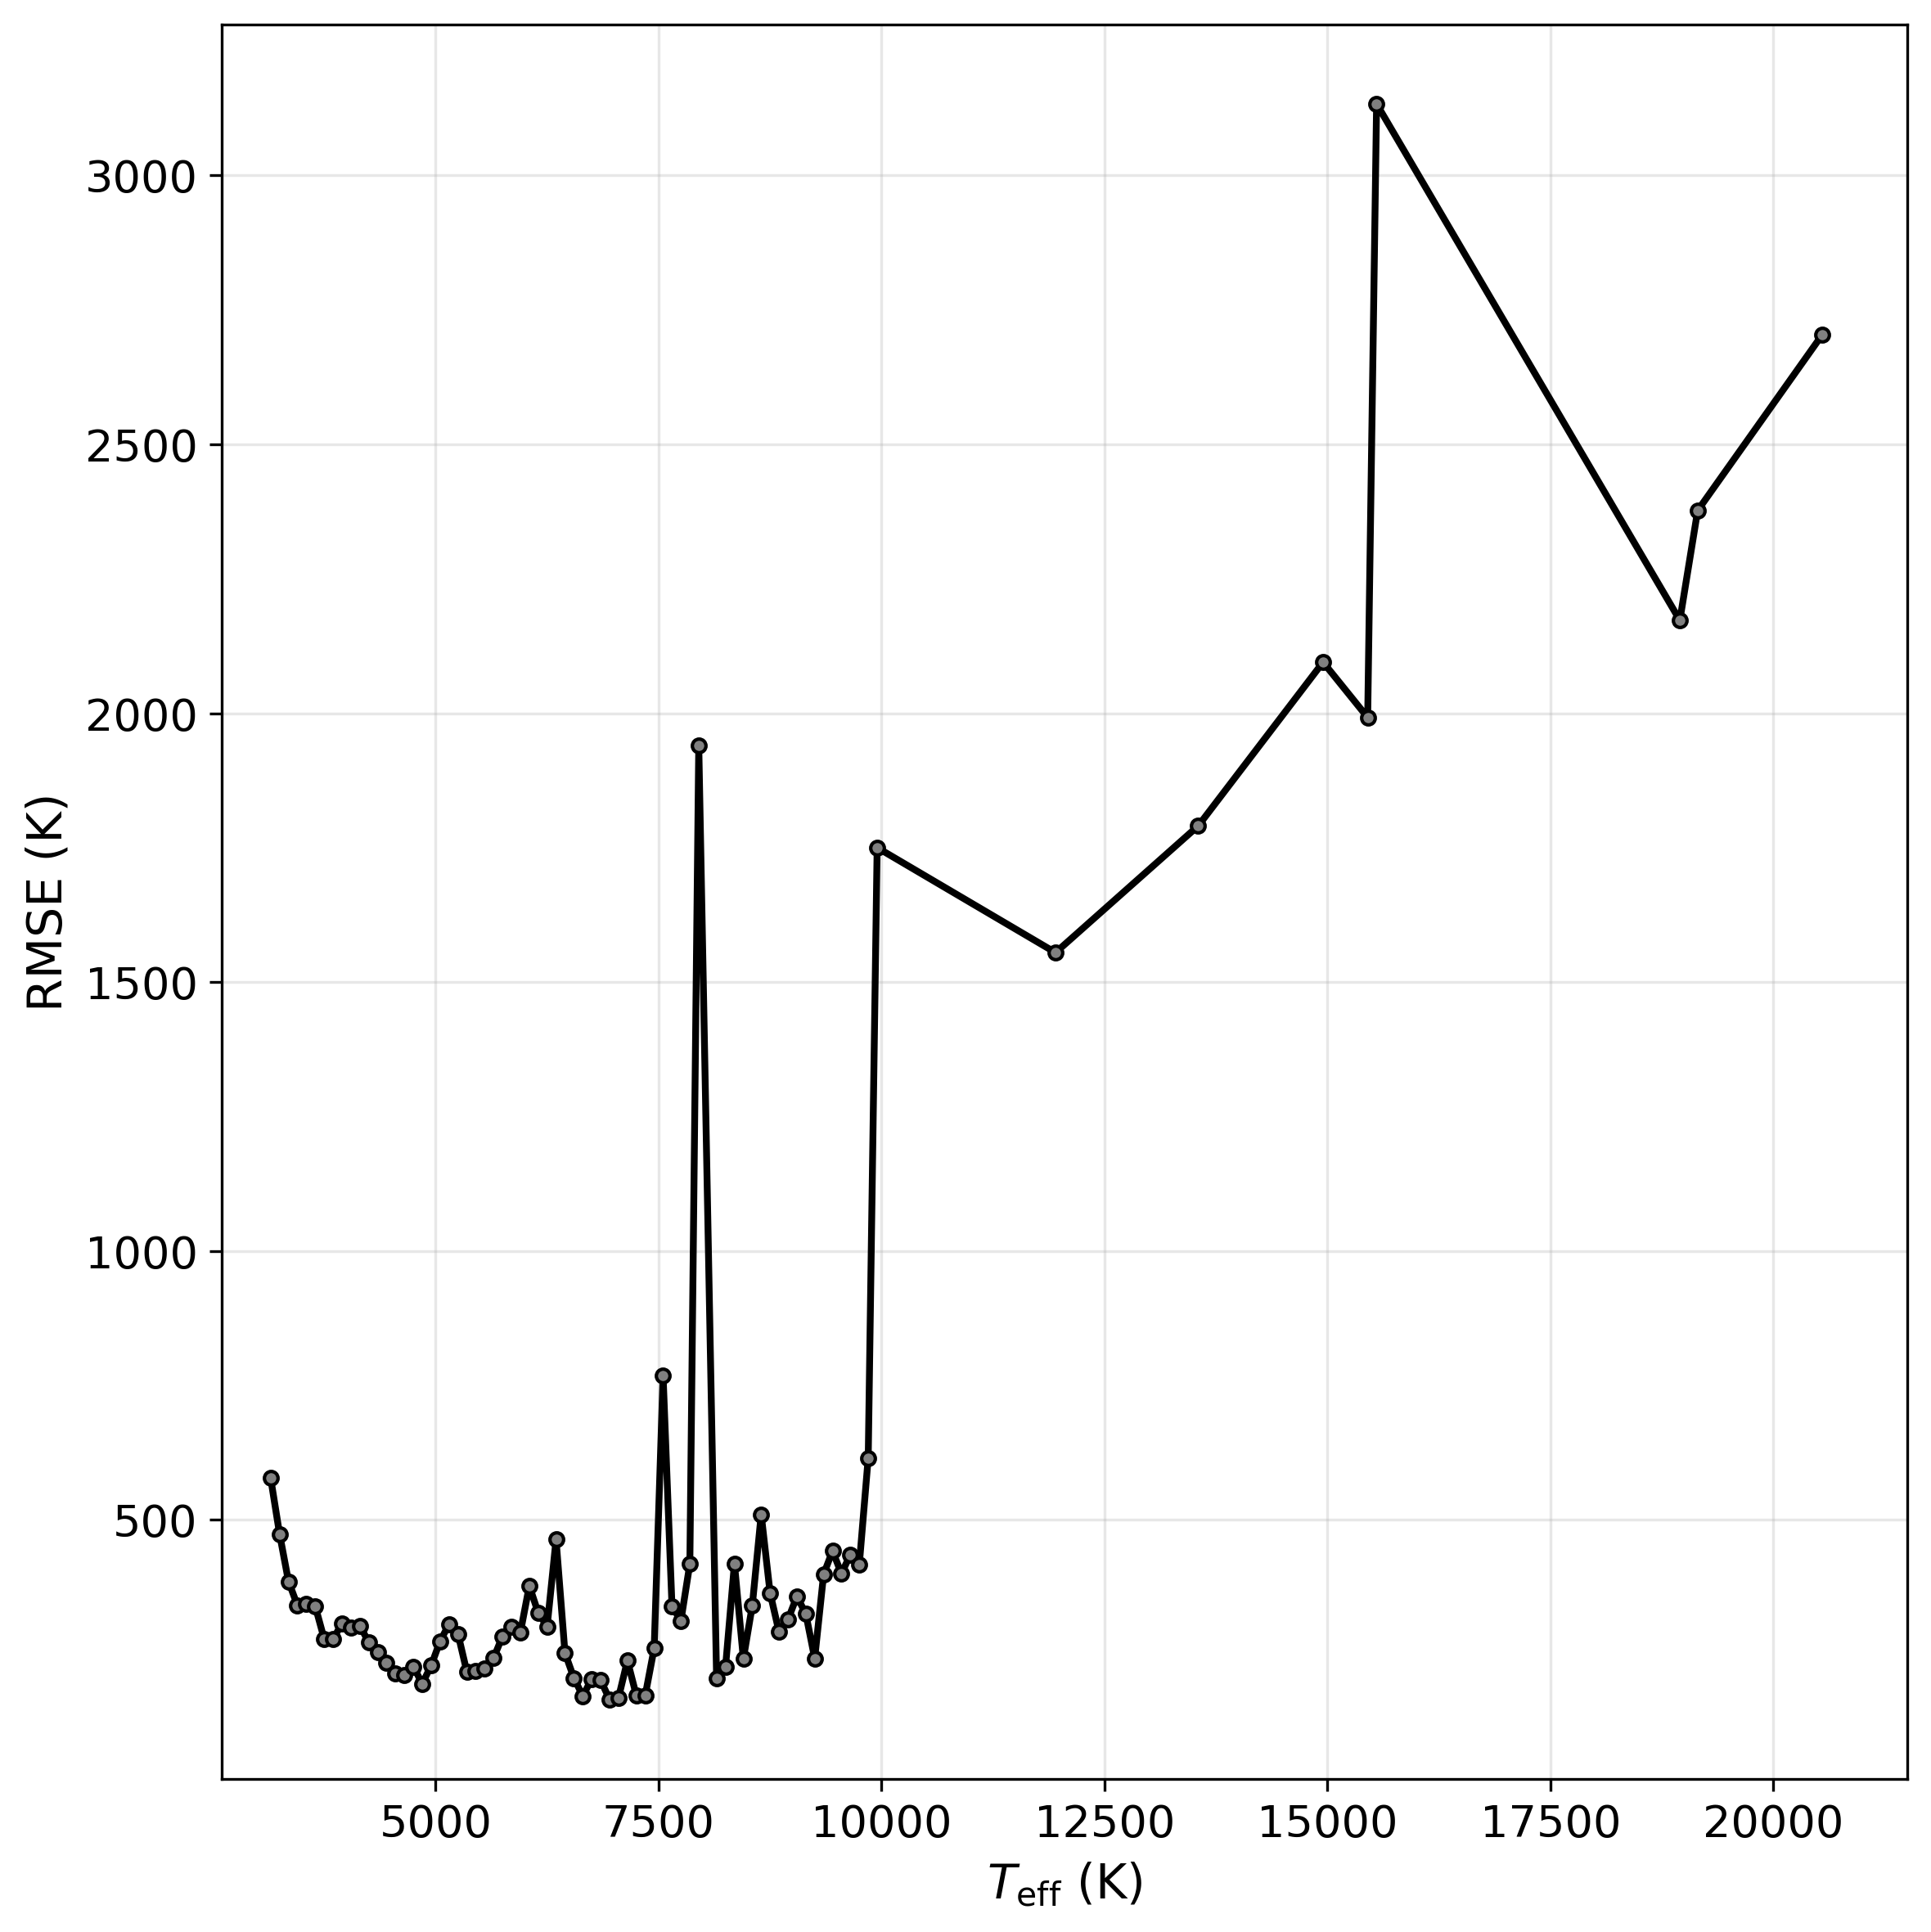
\includegraphics[width=\linewidth]{rmse_by_temperature_line.png} % Replace with third plot
        \label{fig:plot3}
    \end{minipage}\hfill
    \begin{minipage}{0.48\textwidth}
        \centering
        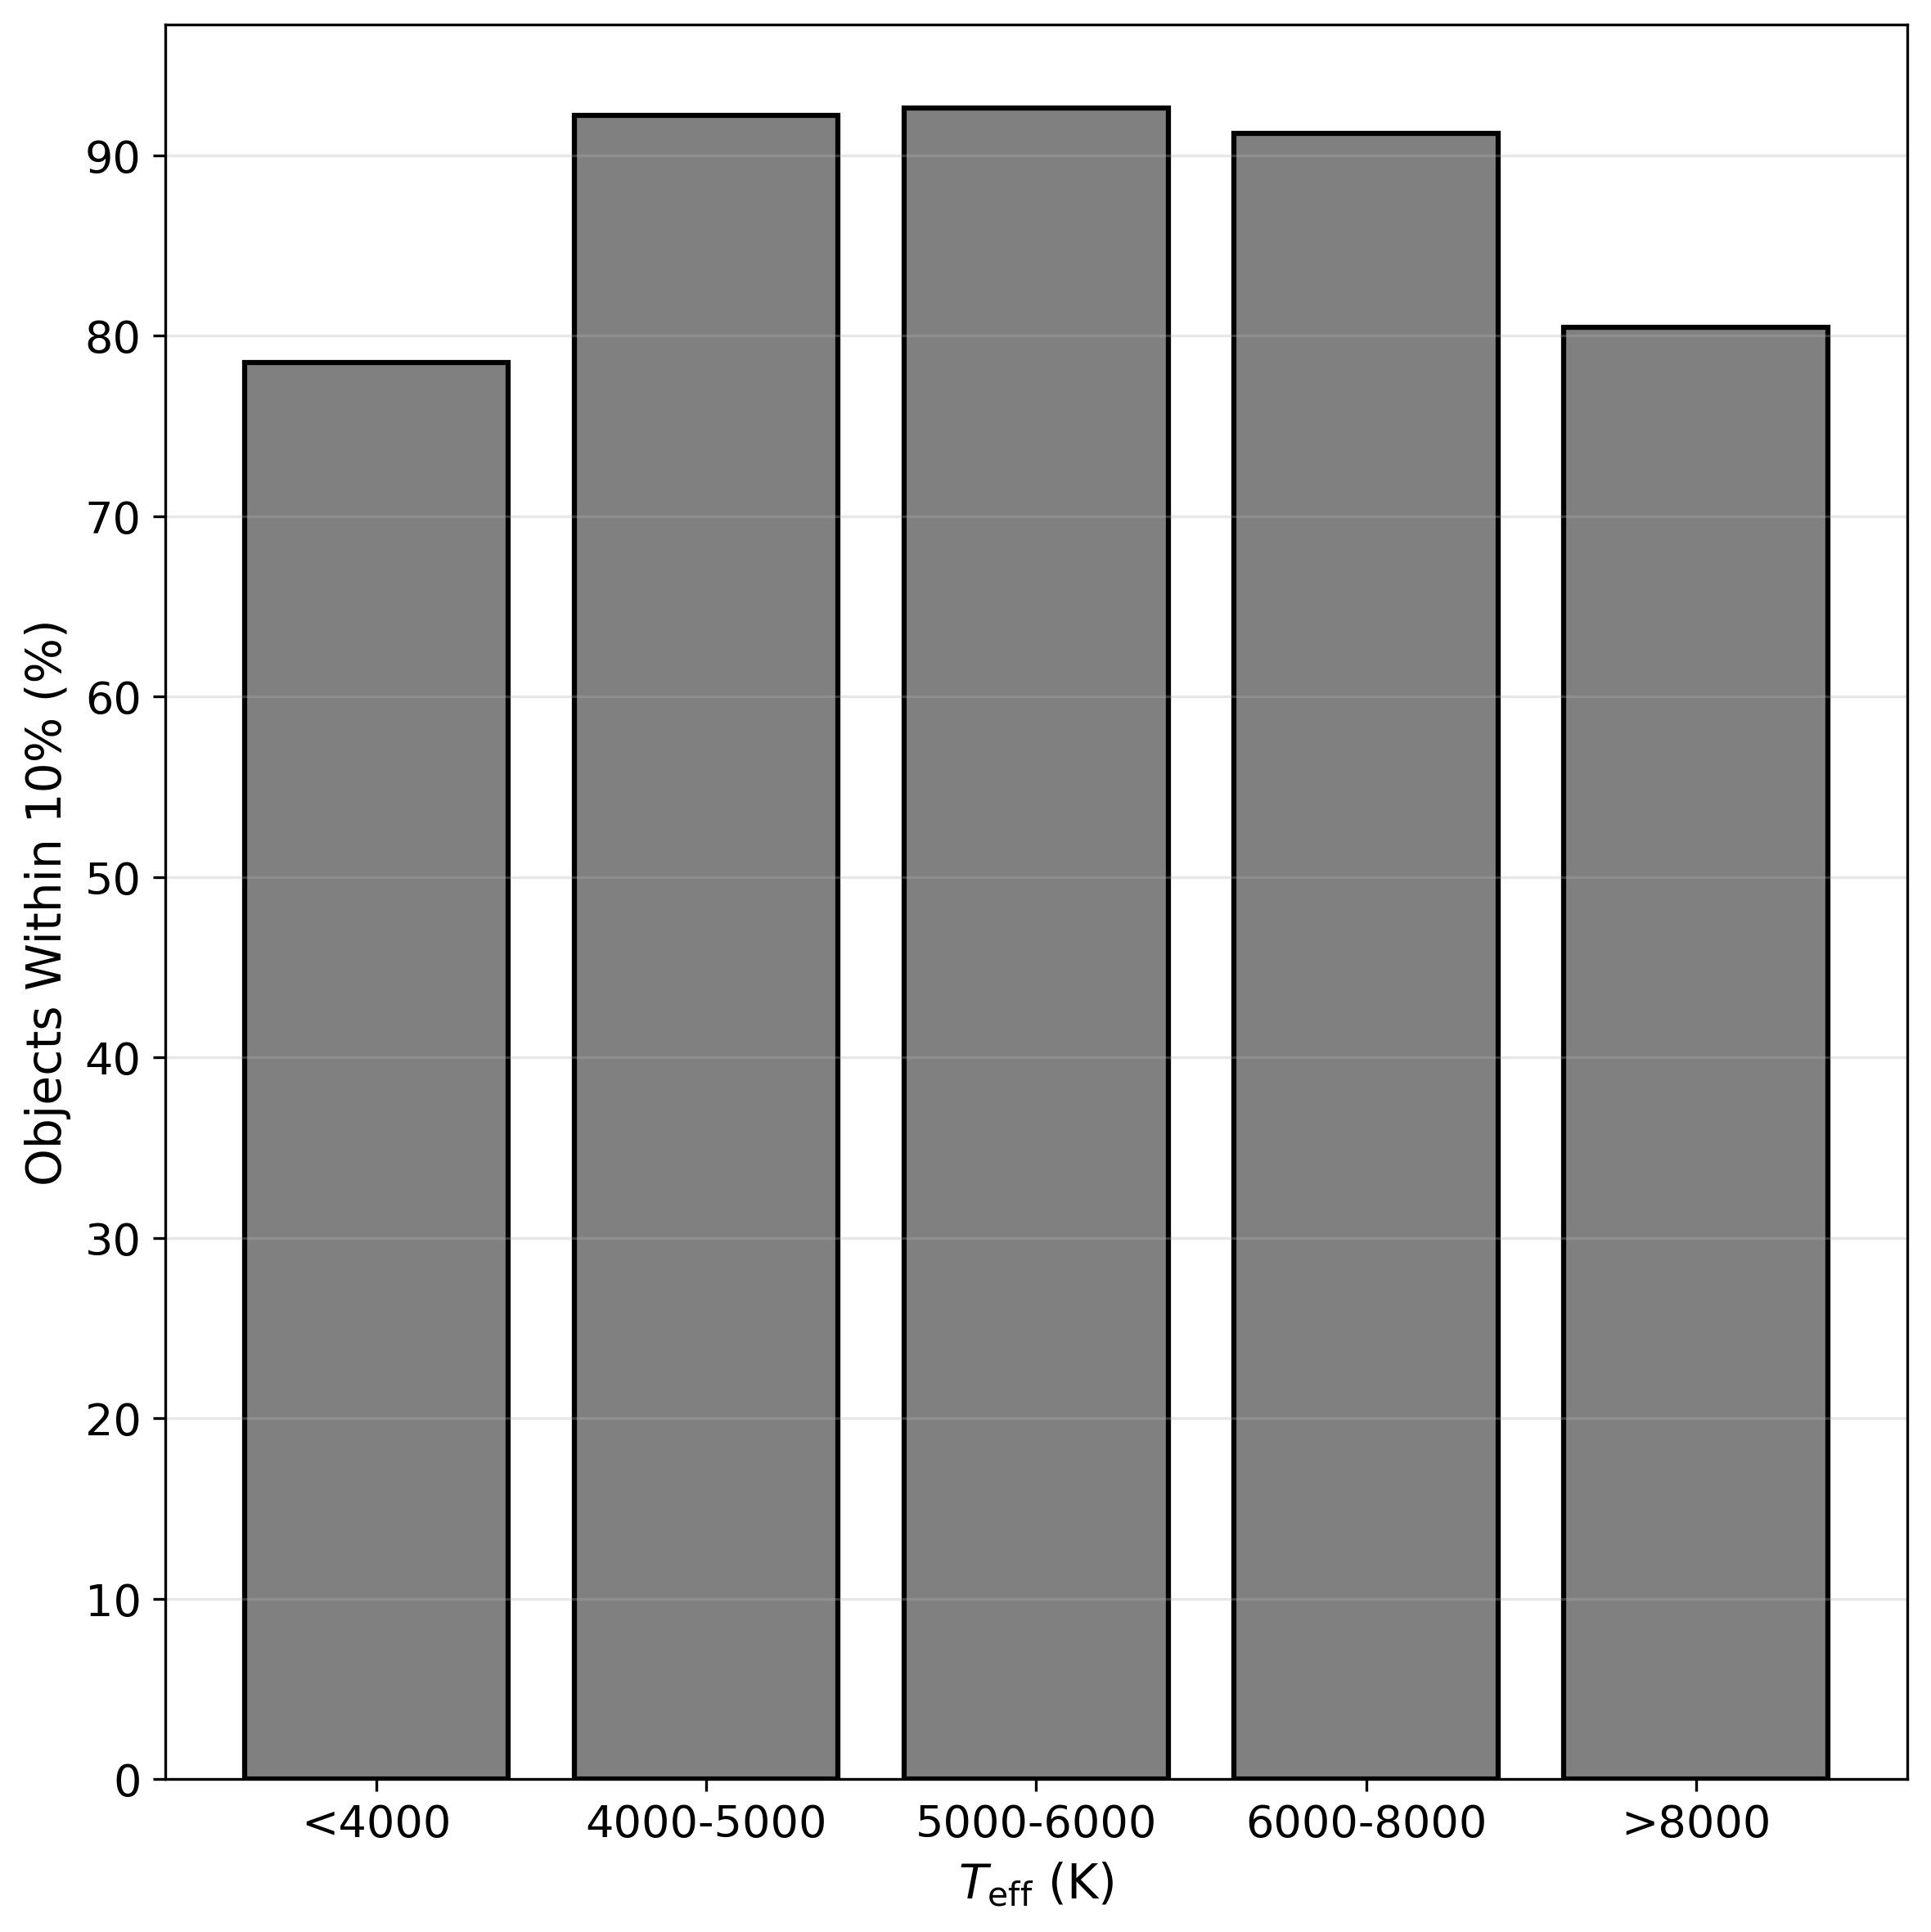
\includegraphics[width=\linewidth]{percentage_within_10pct.png}
        \label{fig:plot4}
    \end{minipage}
    \caption{Validation plots of model performance. 
    Top-left: Feature importance ranking derived from the Random Forest model. 
    Top-right: Density scatter plot of predicted vs. true (GSP-Phot) temperatures; the dashed line represents the 1:1 relation, while dotted lines indicate $\pm 10\%$ error margins. 
    Bottom-left: RMSE as a function of temperature, showing increased uncertainty for hotter stars. 
    Bottom-right: Percentage of test objects with predictions within 10\% of the true value across temperature bins.}
    \label{fig:four_panel_comparison}
\end{figure}

\section{The "Best-of-Four" Ensemble}
\label{sec:ensemble}

\begin{itemize}
    \item \textbf{Internal Uncertainty Estimation:} Using Random Forest variance/quantile spread.
    \item \textbf{Selection Mechanism:} Dynamic selection of the model with the lowest uncertainty per object.
    \item \textbf{Rationale:} Different models perform better in different regimes (e.g., Logg model for giants, Clustering model for complex color regions).
\end{itemize}

\section{Results and Validation}
\label{sec:results}

\begin{itemize}
    \item \textbf{Model Comparison:} Statistical performance (MAE, RMSE, $R^2$) of the three approaches on the test set.
    \item \textbf{Ensemble Performance:} Demonstration of uncertainty reduction and outlier mitigation.
    \item \textbf{Catalog Characteristics:} Distribution of the final predicted temperatures.
    \item \textbf{Validation against "Gold Standard" subsets:} Performance on high-quality literature EBs.
\end{itemize}

\section{Conclusion}
\label{sec:conclusion}

\begin{itemize}
    \item Summary of the "Best-of-Three" methodology.
    \item Impact on the field (availability of the catalog).
    \item Future work (e.g., inclusion of time-series features).
\end{itemize}


%% The Appendices part is started with the command \appendix;
%% appendix sections are then done as normal sections
\appendix

\section{Feature Importance Plots}
\label{app:features}

\section{Uncertainty Validation}
\label{app:uncertainty}

%% If you have bib database file and want bibtex to generate the
%% bibitems, please use
%%
\bibliographystyle{elsarticle-harv} 
\bibliography{references}

%% else use the following coding to input the bibitems directly in the
%% TeX file.

%%\begin{thebibliography}{00}
%% \bibitem[Author(year)]{label}
%% Text of bibliographic item
%%\end{thebibliography}

\end{document}

\endinput

